% -- NAO MUDAR O TAMANHO DA FONTE.
% -- O USO DO TAMANHO DA FONTE EM 12PT Eh OBRIGATORIO
\documentclass[12pt]{article}

% -- O USO DO TEMPLATE DA SBC Eh OBRIGATORIO
% -- NAO ALTERAR NENHUMA PARAMETRO DO MODELO DA SBC
% -- (E.G., MARGENS LATERAIS, RODAPE, CABECA�HO, ENTRE OUTROS)
\usepackage{sbc-template}

\usepackage{graphicx,url}
\usepackage{float}

%\usepackage[brazil]{babel}
\usepackage[latin1]{inputenc}

% descomente abaixo caso tenha problemas com a numera��o das se��es n�o
% aparecerem. Em especial no Ububtu 16.x
%\usepackage{etoolbox}
%\makeatletter
%\patchcmd{\ttlh@hang}{\parindent\z@}{\parindent\z@\leavevmode}{}{}
%\patchcmd{\ttlh@hang}{\noindent}{}{}{}
%\makeatother

% -- O USO DESTE COMANDO Eh OBRIGATORIO
\sloppy

% -- CERTIFIQUE-SE DE QUE O TITULO NAO ESTEJA ULTRAPASSANDO OS LIMITES
% -- DAS MARGENS.
% -- USE O COMANDO QUEBRA-DE-LINHA (\\) SE TITULO FOR MUITO LONGO.
\title{Efficient Visual Attention with Deep Learning}

% -- CERTIFIQUE-SE DE QUE O NOME DOS AUTORES ESTEJA CORRETO.
% -- EM GERAL COLOCA-SE O ALUNO COMO PRIMEIRO AUTOR E O ORIENTADOR COMO
% -- ULTIMO AUTOR.
\author{Erik Perillo\inst{1}, Esther Luna Colombini\inst{1}}

% -- CERTIFIQUE-SE DE QUE OS NOMES DAS INSTITUICOES E SEUS RESPECTIVOS ENDERECOS
% -- NAO ESTEJAM ULTRAPASSANDO OS LIMITES DAS MARGENS. SE ISTO OCORRER, USE O
% -- COMANDO QUEBRA-DE-LINHA (\\) OU ABREVIACOES APROPRIADAS.
\address{Institute of Computing (IC) -- University of Campinas
  (Unicamp)\\
  Caixa Postal 6176 -- 13.084-971 -- Campinas -- SP -- Brazil
  \email{erik.perillo@gmail.com, esther@ic.unicamp.br}
}


% -- CERTIFIQUE-SE DE QUE AS TABELAS E FIGURAS INSERIDAS NO
% -- DOCUMENTO NAO ESTEJAM ULTRAPASSANDO
% -- OS LIMITES DAS MARGENS.

\begin{document}

\maketitle

% -- O RESUMO EM INGLES Eh OBRIGATORIO,
% -- INDEPENDENTE DO IDIOMA EM QUE TRABALHO FOI ESCRITO
\begin{abstract}
The high volume of visual data contains information that is
mostly irrelevant for intelligent agents.
Humans realize sensorial filtering by what we call attention.
We propose a new fully convolutional neural network with relatively
simple architecture for a visual salience system that behaves
similarly to humans, yielding a performance level consistently among the
best ten state of the art models in MIT300 benchmark while having around
three times less parameters than others.
\end{abstract}

% -- O RESUMO EM PORTUGUES Eh OBRIGATORIO, INDEPENDENTE DO
% -- INDIOMA EM QUE O TRABALHO FOI ESCRITO
\begin{resumo}
A alta quantidade de dados visuais cont�m informa��o que � em sua maior
parte irrelevante para agentes inteligentes.
Nos seres humanos, h� um filtro sensorial realizado pela aten��o.
Propomos uma nova rede neural totalmente convolucional com arquitetura
relativamente simples para um sistema de sali�ncia visual que se comporta
similarmente a humanos,
com um desempenho que a coloca consistentemente entre os dez
melhores modelos estado da arte no \tit{MIT300 benchmark} com cerca de
tr�s vezes menos par�metros que outros.
\end{resumo}

\section{Introduction}
One of the most challenging unsolved problems in Artificial Intelligence is
vision.
It is fundamental for the conception of systems that interact with the real,
physical world.
Such systems would be useful for applications that involve
robotics and tasks in domestic houses, industry and agriculture, so
there is great potential for the benefit of society.

Vision is remarkably data and computationally intensive:
In humans, approximately half the brain is involved in
vision-related tasks~\cite{fixott_1957}.
Even our minds can't handle all the sheer amount of sensorial information
received every second: We have attention, a fundamental mechanism
that, among other functionalities, filters out irrelevant information
-- either visual or from other senses-- and helps us focus our cognitive
processes on what is important at a given moment.
These facts are a strong evidence that, in order to solve
vision, we need to have attention.

\subsection{What is visual saliency?}
Visual saliency can be defined as the delimitation of a certain spatial
region on an image for further cognitive processing~\cite{treisman_1980}.
The phenomenon may emerge from two fundamentally different processes:
There is \emph{top-down} attention, an internal
stimuli of the agent (e.g. find a red apple in a tree because of hunger,
which will automatically make red be reconizable more easily on the scene),
and \emph{bottom-up} attention, an external process which captures the
agent's attention from abrupt changes in visual stimuli or high contrast.
In this work, we focus on \emph{bottom-up} attention.
\begin{figure}[hbt]
\begin{center}
		\begin{tabular} {cc}
		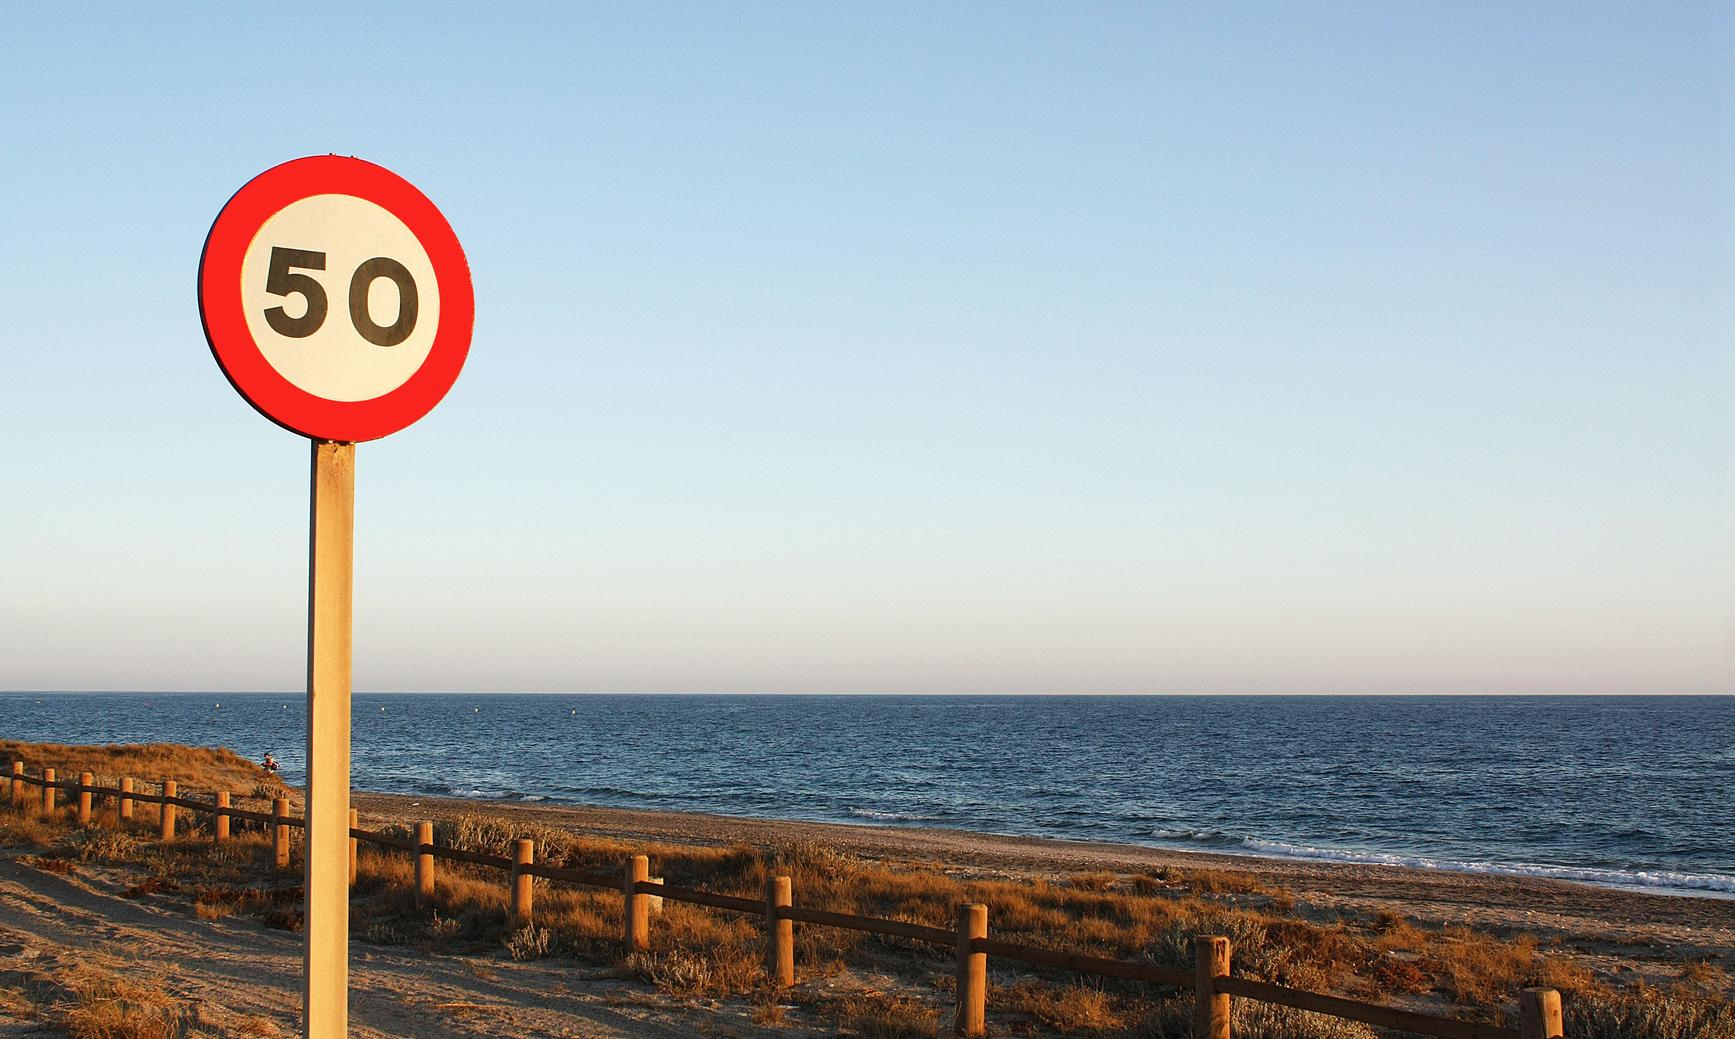
\includegraphics[width=0.39\textwidth]{./img/traffic_sign_s.jpg} &
		
\includegraphics[width=0.39\textwidth]{./img/traffic_sign_m.jpg}\\
        (a) & (b)
		\end{tabular}
\end{center}
\caption{Example of visual saliency.
    b) is the salience map where brighter pixels represent regions more
    salient to humans on the original image a).}
\label{fig:example}
\end{figure}

Visually salient regions on images are usually represented by
\emph{saliency maps}.
Such maps are grayscale images generated such that
areas with pixels close to white express high saliency
of the same region on the original image, whereas regions with pixels close
to black represent a region of low saliency.
Datasets with pairs image-map are usually obtained by colleting eye-fixation
data from humans that looked at the images.

\subsection{Related work}
Early computational models of visual saliency were generally built based on
filtering of images for extraction of a pre-selected set of features
considered important for \emph{bottom-up} attention.
\emph{Vocus}~\cite{frintrop_2005} is a computational model that extracts
features shown to be naturally salient to humans such as color/luminance
contrast and orientation~\cite{colombini_2016} from different scales of the
image.

A rapid change of paradigm ocurred around 2015 when \emph{Deep Learning}
techniques showed to be extremely effective in the generation of saliency
maps.
Models such as \emph{Salicon}~\cite{jiang_2015} showed that applying
convolutional neural networks with weights initialized from networks used
for image classification, e.g. \emph{VGG-16}~\cite{zisserman_2014}
could yield maps very similar to those generated from humans.
\emph{ML-Net}~\cite{cornia_2016} uses the output from different layers
of \emph{VGG-16} to use information from various dimensions and levels of
abstraction.
\emph{DeepFix}~\cite{kruthiventi_2015} extends a pre-trained model with
new layers that account for global features and center bias.
\emph{Salnet}~\cite{pan_2016} is a work that explores two models that are
simple yet provide good results.
Models are usually evaluated and ranked on
\emph{MIT saliency benchmark}~\cite{mit_sal_bm}, which uses a variety of
metrics to express how close generated saliency maps are to those created from
human data.
As of today, at least nine out of the ten best models in the ranking use
Deep Learning.

\subsection{Motivation}
Current state of the art models are in general quite expensive computationally,
partly because most of them are based on very big pre-trained networks.
The convolutional layers of \emph{VGG-16} are composed of around 14.7
million parameters.
While pre-trained weights from classification tasks showed to be effective
for saliency prediction, it is reasonable to question whether
creating a proper network from scratch could yield a smaller amount of
parameters that are more efficient for the sole task of salience prediction.
Also, there are some ideas from previous work on psychology that weren't
found to be used in current models but are considered worthwhile to be
explored.

\subsection{Objectives}
This work aims at building a visual saliency model that is a) effective,
yielding results similar to other state of the art models,
and b) relatively simple and computationally efficient.
It is important that both criteria are matched because we aim at extending the
model in the future for video and real time applications such as
navigating robots.

\section{Proposed model}
Figure~\ref{fig:model} illustrates the overall architecture of our fully
convolutional neural network.
It extracts features from increasingly smaller dimensions of the
input image.

\begin{figure}[hbt]
    \centering
    \def\svgwidth{\columnwidth}
    \input{./img/model.pdf_tex}
    \label{fig:model}
    \caption{Overview of the network.
        Filters sizes are in format width$\times$height\_stride.}
\end{figure}

The network is composed of four main blocks:
\begin{enumerate}
    \item First level extracts low level features from the input image, of
        dimensions $W\times H \times 3$ (width, height, depth), using
        a single layer with 48 convolution filters with ReLu activation
        followed by max-pooling that reduces image by a factor of two.
        It was found that further decreasing the number of filters in this
        layer considerably hurts performance, which makes sense because it is
        important to capture high spatial frequency and high contrast
        information in the context of visual saliency.
    \item Second level extracts low-medium level features from the
        input of dimensions $W/2 \times H/2 \times 48$ using two layers
        with 64 and 96 convolution filters, respectively, followed by ReLU
        activation and max-pooling.
    \item Third level extracts medium-high level features from input with
        dimensions $W/4 \times H/4 \times 96$ using four convolution layers.
        The first two have 128 filters each, the last two have 144 filters
        each. Every convolution layer is followed by ReLu.
        Max-pooling is realized at the end.
        A considerable depth in this level was found to be important for
        the networks performance.
    \item Fourth and last level is composed of eight inception blocks
        that extract high level features from the input with
        dimensions $W/8 \times H/8 \times 144$.
        Great level of depth and Inception blocks were found to be very
        important at this level.
        A $1 \times 1$ convolution makes a linear combination of the output
        maps at the end of the 8 inception blocks, followed by ReLu, producing
        the final saliency map of dimensions $W/8 \times H/8 \times 1$.
\end{enumerate}

\begin{figure}[H]
    \centering
    \def\svgwidth{0.60\linewidth}
    \input{./img/inception.pdf_tex}
   \label{fig:inception}
    \caption{Inception block layout.}
\end{figure}

Figure~\ref{fig:inception} illustrates the inception
architecture~\cite{szegedy_2014}
used in each block: We use filters of size $5 \times 5$, $3 \times 3$
(both preceeded by $1\times 1$ convolutions in order to reduce number
of input filters), $1 \times 1$, and a max-pooling of size $3 \times 3$.
Each of these operations is realized in parallel from the same input
and the outputs are concatenated at the output.
Inception allows the network to use
information from different spatial dimensions as well as previous
layers (lower level saliency information) in the final map
computation, which is considered to be important for visual saliency.
The network has a total of $3717841$ parameters, a very low number
compared to other models.

\begin{table}[H]
\centering
\label{table:inception}
\caption{Number of filters used in each inception block.}
\begin{tabular}{|c|c|c|c|c|c|c|}
	\hline
    Block & pool & conv 1$\times$1 & 3$\times$3 reduce &
    conv 3$\times$3 & 5$\times$5 reduce & conv 5$\times$5\\
    \hline
    1 & 96 & 128 & 96 & 192 & 58 & 96\\
    \hline
    2 & 64 & 128 & 80 & 160 & 24 & 48\\
    \hline
    3 & 64 & 128 & 80 & 160 & 24 & 48\\
    \hline
    4 & 64 & 128 & 96 & 192 & 28 & 56\\
    \hline
    5 & 64 & 128 & 96 & 192 & 28 & 56\\
    \hline
    6 & 64 & 128 & 112 & 224 & 32 & 64\\
    \hline
    7 & 64 & 128 & 112 & 224 & 32 & 64\\
    \hline
    8 & 112 & 160 & 128 & 256 & 40 & 80\\
    \hline
\end{tabular}
\end{table}

\subsection{Implementation}
We used \emph{Theano} \texttt{0.9.0.dev}
along with \emph{Lasagne} \texttt{0.2.dev1}
on a machine with \emph{Ubuntu 16.04 LTS} and
kernel \emph{Linux} \texttt{4.8.0-54-generic}.
Training was conducted on a GPU \emph{NVIDIA GTX 1080}.
Code is available at \texttt{https://goo.gl/WzpyYJ}.

\subsection{Training}
We resize images to dimensions $320\times240\times3$ during training.
Each image is normalized channel-wise subtracting the channel mean and
dividing by the standard deviation.
We consider normalizing per image, rather than per dataset,
to be more reasonable because visual
saliency is highly connected to the context of the image.
We also convert the images to the LAB colorspace.
\emph{Vocus}~\cite{frintrop_2005} cites that the LAB colorspace is more
closely related to human vision by encopassing red-green, yellow-blue and
luminance maps. We conjecture that this colorspace facilitate extraction of
important luminance and color contrasts by the learned convolution filters.
Our prior tests showed better performance using image-wise
normalization and LAB instead of the commonly used RGB\@.

We aimed at maximizing (or minimizing the negative) of the
\emph{Correlation Coefficient} of the ground-truth saliency map $G$ and
the predicted map $P$:
$CC(P, G) = cov(P, G)/(\sigma(P)\sigma(G))$.
There is a variety of metrics for evaluating saliency
predictions~\cite{judd_2016}, but we consider $CC$ to be the most appropriate
because it simmetrically penalizes both false positives and false negatives.

We considered two datasets for training:
\emph{SALICON}~\cite{jiang_2015}, with 15000 images, and
\emph{Judd}~\cite{judd}, with 1003 images.
The network was trained using Stochastic Gradient Descent with Nesterov
Momentum of $0.9$.
We first used SALICON with data augmentation by flipping images
horizontally and vertically and the target normalized by mean-std
(Last conv layer had ReLu removed in this step).
We first used mean-std normalization
of targets because it was noted that it allowed for a faster convergence.
Training iterated for 5 epochs with learning rate of $0.009$
and then for 3 epochs with learning rate of $0.001$.
We then switched to using unit normalization on targets.
The network was trained for 1 epoch with learning rate of
$3\times10^{-5}$ and L2 regularization of $10^{-4}$.
Finally, we used Judd with data augmentation by flipping images horizontally
and the target normalized by unit normalization.
Training iterated for 2 epochs with learning rate of
$5\times10^{-5}$ and L2 regularization of $3\times10^{-5}$.
Batch sizes were 10 for SALICON and 2 for Judd.
The whole training process took around two and a half hours.

\section{Results}
\begin{figure}[hbt]
\begin{center}
		\begin{tabular} {ccc}
        Stimulus & Ground-truth & Ours\\
		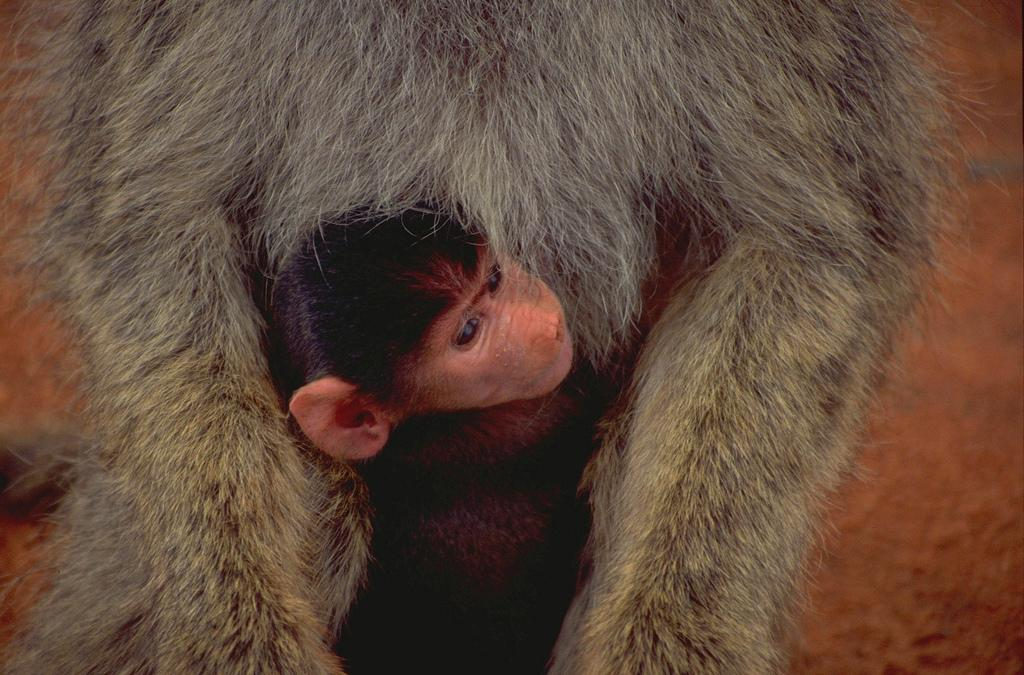
\includegraphics[width=0.21\textwidth]{./img/monkey_s.jpg} &
        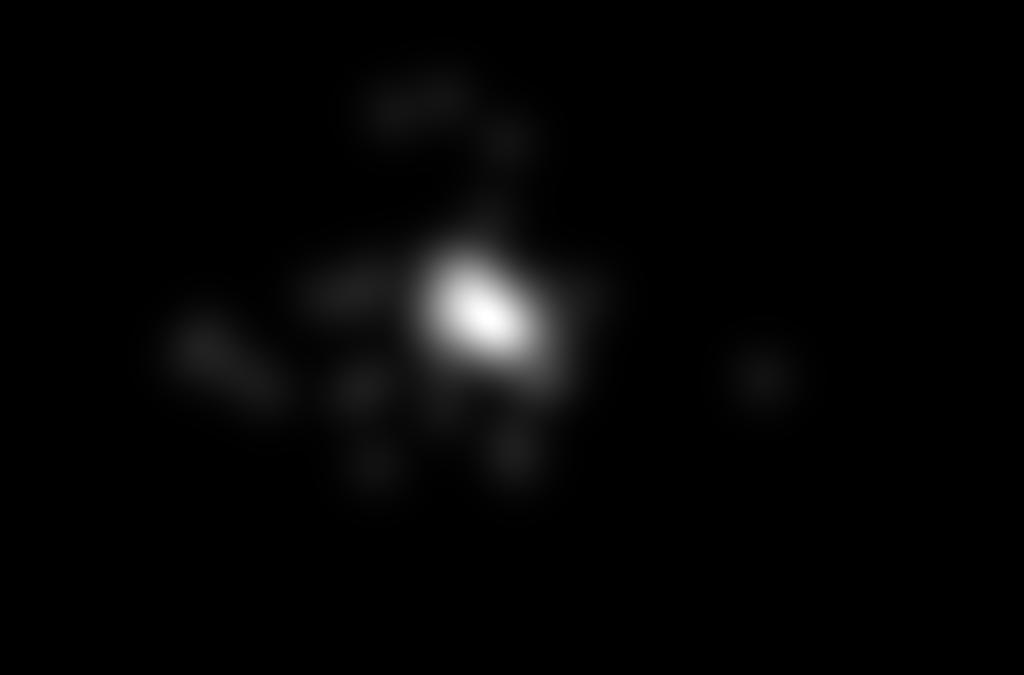
\includegraphics[width=0.21\textwidth]{./img/monkey_gt.jpg} &
		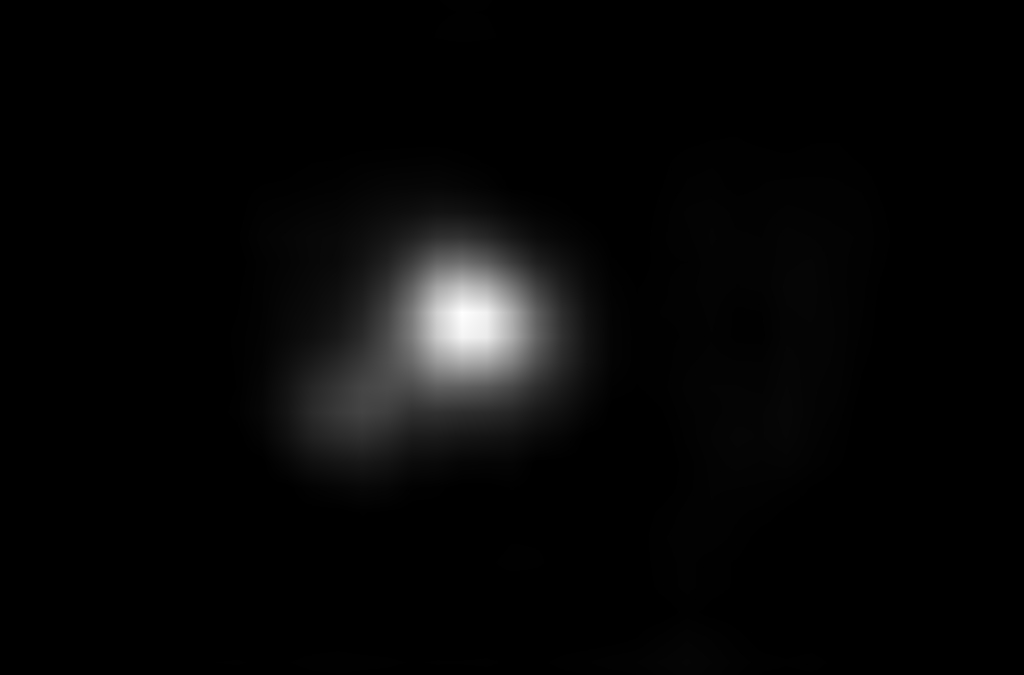
\includegraphics[width=0.21\textwidth]{./img/monkey_m.jpg}\\
		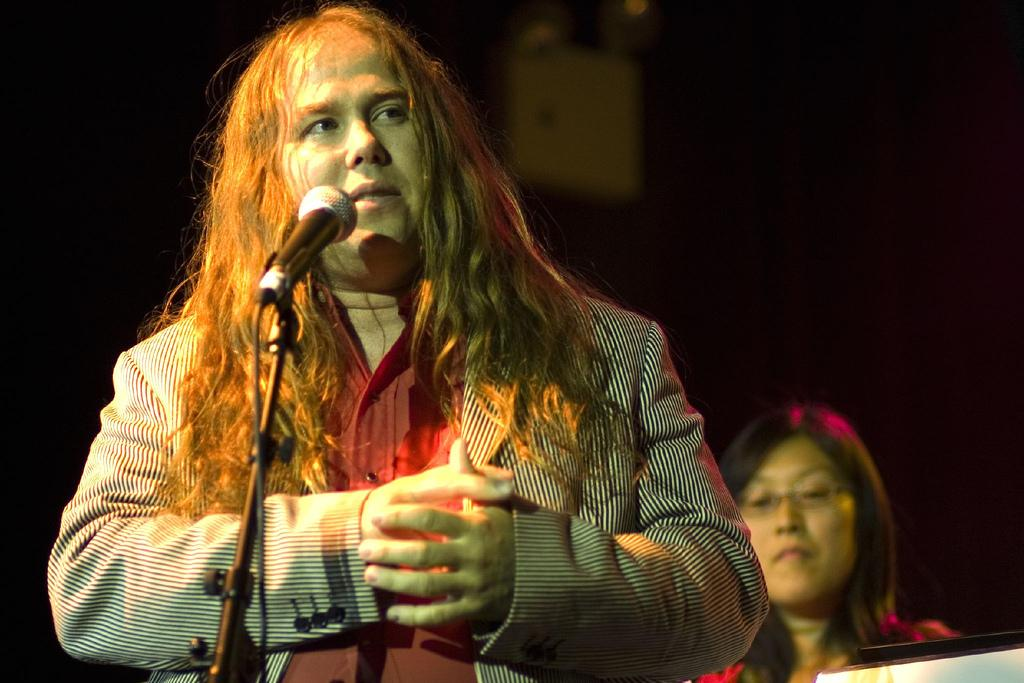
\includegraphics[width=0.21\textwidth]{./img/person_s.jpg} &
        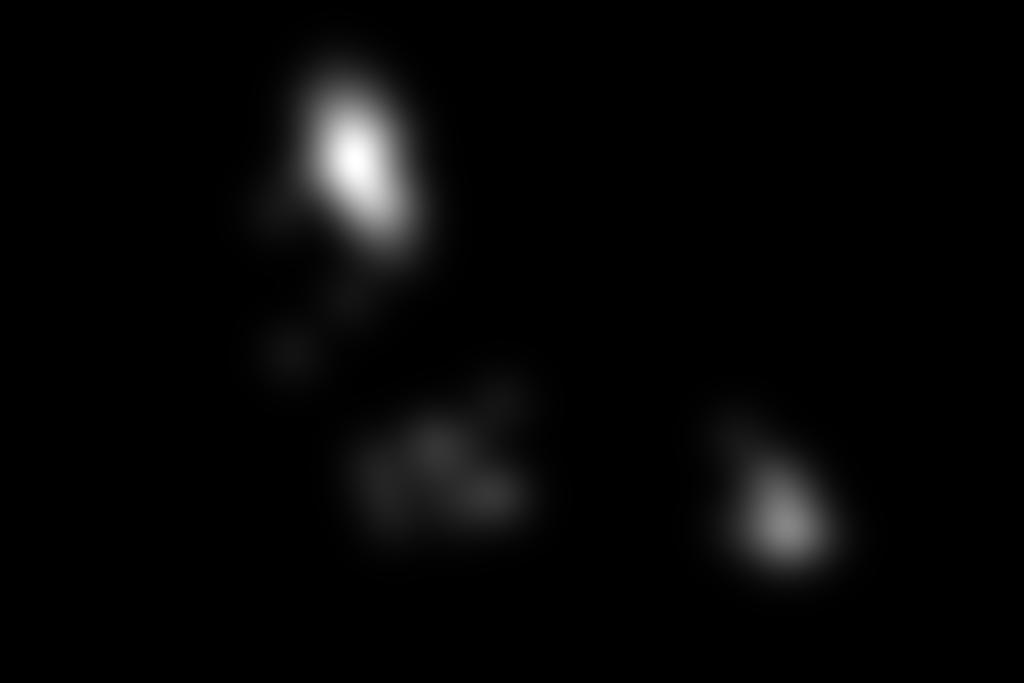
\includegraphics[width=0.21\textwidth]{./img/person_gt.jpg} &
		
\includegraphics[width=0.21\textwidth]{./img/person_m.jpg}\\
		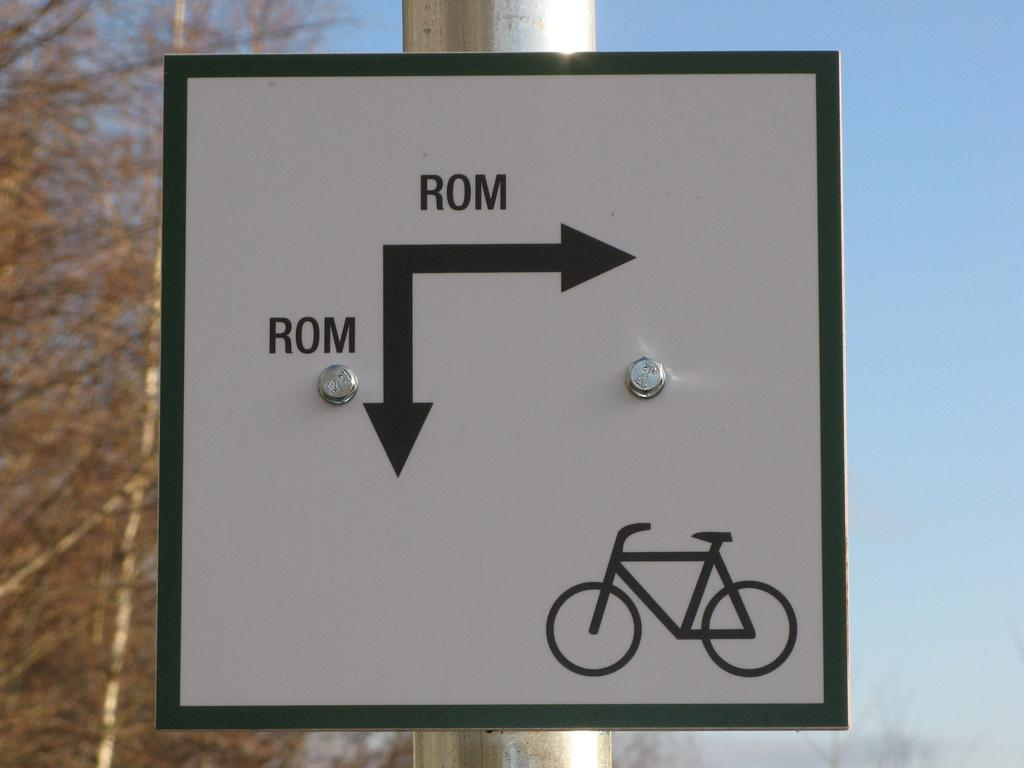
\includegraphics[width=0.21\textwidth]{./img/sign_s.jpg} &
        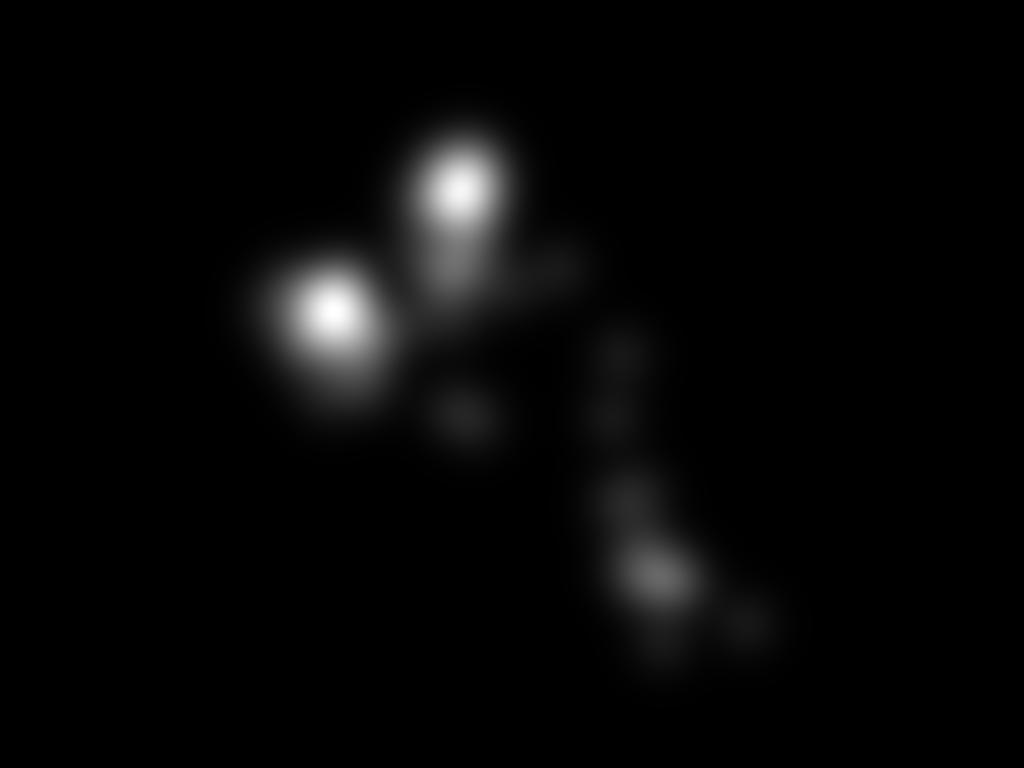
\includegraphics[width=0.21\textwidth]{./img/sign_gt.jpg} &
		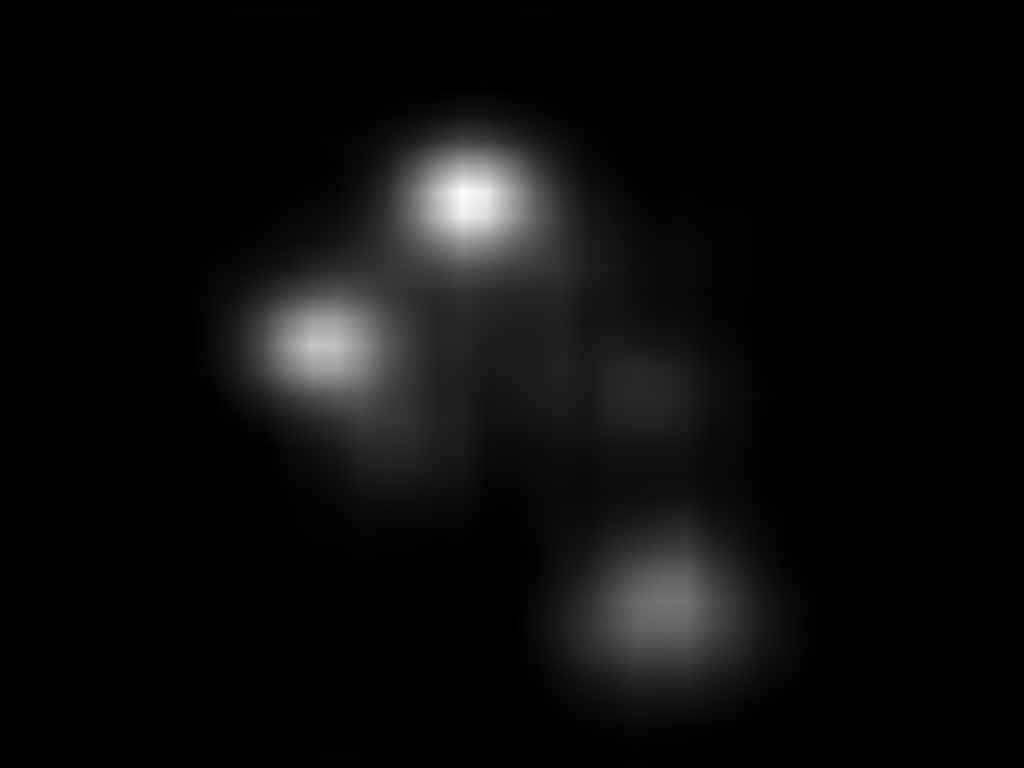
\includegraphics[width=0.21\textwidth]{./img/sign_m.jpg}\\
		\end{tabular}
\end{center}
\caption{Examples of predictions made by our model.}
\label{fig:preds}
\end{figure}

\begin{table}[H]
    \centering
    \label{table:results}
    \caption{State of the art models and metric scores on
    \emph{MIT300 benchmark}.}
    \begin{tabular}{|c|c|c|c|c|c|c|}
        \hline
        \tbf{Model} & Num. parameters & AUC-Judd $\uparrow$ & CC $\uparrow$
            & NSS $\uparrow$ & Sim $\uparrow$ & EMD $\downarrow$\\
        \hline
        Infinite humans & - & 0.92 & 1.0 & 3.29 & 1.0 & 0\\
        \hline
        \emph{DeepFix} & $\approx$16.7 million & 0.87 & 0.78
            & 2.26 & 0.67 & 2.04\\
        \hline
        \emph{Salicon} & $\approx$14.7 million & 0.87 & 0.74 & 2.12
            & 0.60 & 2.62\\
        \hline
        \textbf{Ours} & \textbf{3.72 million} & \textbf{0.85} &
        \textbf{0.71} & \textbf{1.98} & \textbf{0.62} & \textbf{2.37}\\
        \hline
        \emph{ML-Net} & $\approx$15.4 million & 0.85 & 0.69 & 2.07 & 0.60
            & 2.53\\
        \hline
        \emph{SalNet} & 25.8 million & 0.83 & 0.57 & 1.51 & 0.52 & 3.31\\
        \hline
    \end{tabular}
\end{table}

Predition took an average time of 8 milliseconds.
Figure~\ref{fig:preds} show some maps generated by our model.
They are generally considerably similar to the ground truth.
We tested our model on the 300 images of the \emph{MIT300 benchmark}.
Table~\ref{table:results} shows the results,
metrics in bold show our values.
Our model achieves results comparable to the best state of the art models,
while having at least one fourth of the number of parameters.

\section{Conclusion}
In this paper, we proposed a novel fully convolutional neural network for the
prediction of visual saliency on images.
Our model architecture and data preprocessing were designed specifically
for the task of salience prediction.
Our methods showed to be very effective, yielding a network with performance
on \emph{MIT300 benchmark} consistently among the ten best results on various
metrics while having around three times less parameters than other state of
the art models.

% -- NAO MUDAR O ESTILO DAS REFERENCIAS BIBLIOGRAFICAS. O USO DO PADRAO DA SBC Eh OBRIGATORIO
\bibliographystyle{sbc}
\bibliography{sbc-template}

\end{document}
